\section{Izmantošana pasaulē}

Silīcija Saules paneļu attīstības intensīvākais posms bija apmēram no 1980. līdz 2000. gadam, kad to maksimālā efektivitāte palielinājās no 15\% līdz 25\%
\cite{Sivaram}. Nākamajos 20 gados efektivitātes pieaugums bija gandrīz desmit reizes mazāks. Tiek pētīti arī citi Saules paneļu pusvadītāju veidi, piemēram, kadmija telurīda (\textit{cadmium telluride}, CdTe) vai gallija arsenīda (\textit{Gallium arsenide}, GaAs), tomēr monokristāliskā un polikristāliskā Si Saules paneļi joprojām aizņem lielāko daļu no tirgus, piemēram, Vācijā Si sastādīja vairāk nekā 90\% no Saules paneļu tirgus pēdējo septiņu gadu laikā ~\cite{prognoze}. Tas tādēļ, ka Si ir pieejamāks un lētāks nekā GaAs\cite{hayes_clemens_2015}, un vairāk izpētīts nekā CdTe pusvadītāji~\cite{Sivaram}.

Svarīgi ievērot, ka Saules paneļu efektivitāte ir atkarīga no vairākiem faktoriem, kas mainās līdz ar ģeogrāfisko novietojumu: ģeogrāfiskā platuma, gadalaika, mākoņainības un gaisa piesārņojuma. Tātad, detalizēta Saules paneļu efektivitātes analīze var būt noderīga katrā valstī, lai precīzāk izvērtētu solārās enerģijas lietošanas perspektīvas tajā. Var minēt dažus šādu pētījumu piemērus.
\begin{itemize}
  \item Indijas pilsētā Bangalorē izpētīja, ka efektivitāte musona un pēc-musona periodos ir augstāka, nekā ziemā un vasarā. To var saistīt ar lielu nokrišņu daudzumu musona periodā, kas labi dzesē Saules paneļus, un ar lielāku saulaino dienu skaitu pēc-musona periodā~\cite{effectCloudsOnSurface}.
  \item Eksperiments Mumbajā ļauj secināt, ka karsts un sauss klimats ne tikai samazina enerģijas pārvērtības lietderības koeficientu, bet arī izraisa defektus un silīcija bojājumus, kas palielina enerģijas zudumus. Tiek norādīts, ka šādā klimatā tipiskais Saules paneļu dzesēšanas risinājums -- ūdens izsmidzināšana -- nav pielietojams, jo tieši šādā klimatā ūdens trūkums ir svarīga problēma~\cite{improvePerformance}.
  \item Indonēzijā pētnieki novēroja, ka mitruma un vēja ātruma palielināšana samazina Saules paneļu efektivitāti~\cite{improvePerformance}~\cite{Sani_2018}. Atšķirībā no iepriekšējā pētījumā, aplūkotajā temperatūras apgabalā (42 -- 52 \textdegree C) temperatūra pozitīvi korelē ar paneļu efektivitāti, kas, iespējams, saistīts ar GHI palielināšanos. 
  \item Arī Latvijā jau ir uzstādītas saules paneļu sistēmas. Piemēram, Ulbrokā 2017. gadā 20 paneļu sistēma kopā saražoja 4554.06 kWh -- vidēji 227.703 kWh gadā no viena paneļa (skat.~\ref{fig:ulbroka}).
\end{itemize}


\begin{figure}[h]
  \centering
  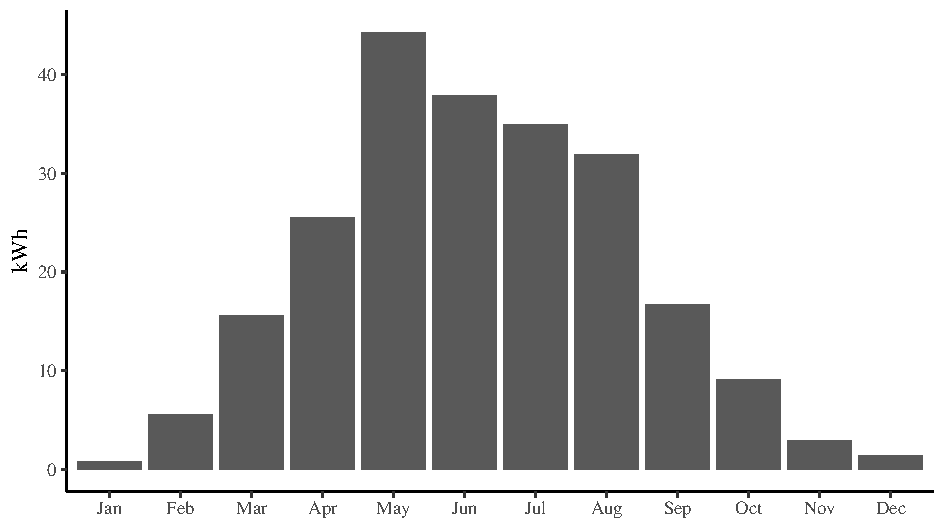
\includegraphics[width=\linewidth]{figures/misc/ulbroka1.pdf}
  \caption{Viena saules paneļa saražotā enerģija Ulbrokas saules paneļu spēkstacijā 2017. gadā. Virziens: D, leņķis 15 \textdegree ~\cite{fronius} (datu nolasīšana: Valts Krūmiņš)}
  \label{fig:ulbroka}
\end{figure}

\section{Darba aktualitāte}

Latvijā veikto pētījumu daudzums un kvalitāte pagaidām neļauj iegūt pilnīgu priekšstatu par Saules paneļu lietošanas iespējām un prognozēt dažādu paneļu tipu efektivitāti reālā Latvijas klimatā. Tāpēc šī darba novitāte ietverta programmatūras izveidē, kas ļauj attēlot un apstrādāt Saules paneļu monitoringa datus, kas dos iespēju veikt turpmākus dziļākus pētījumus par dažādiem solārās enerģijas pielietojuma aspektiem Latvijā.

